\section{Mechanism and Recovery Under Bidirectional Supervision}
\label{sec:cs_mechanism_section}

The previous section established what standard fine-tuning does. This section
asks why the reverse failure takes the form it does, and how much of it explicit
reverse supervision can repair. The evidence supports a deliberately narrow
claim. On lexical transformations the reverse mapping stays accessible at
inference time yet goes unused in the final generation. On harder
transformations, explicit reverse supervision restores structural rewriting but
not semantic recovery.

\subsection{Phenomenology of the Failure}
\label{sec:cs_phenomenology}

Three properties recur across the reverse evaluations. First, reverse recovery
falls to zero in every standard fine-tuning condition we test. Second, prompting
does not rescue the reverse direction. Third, the outputs concentrate at the
obfuscated endpoint rather than drifting randomly through program space. This
third property shows that the model has not become uncertain. It has
become directionally biased toward re-expressing the forward transformation.

The surface outcome is shared across task types, yet the inverse tasks differ in
difficulty. Identifier Renaming is local and lexical. Dead Code Insertion
requires the model to find and delete the semantically inert inserted blocks.
Literal Encryption requires recovery of hidden literal values from the inserted
decryption logic. We therefore read the uniform 0\% reverse recovery as a single
behavioral endpoint reached from increasingly different underlying difficulties.
The distinction returns when we compare recovery under bidirectional and
contrastive training.

For Identifier Renaming, the case for genuine capability loss is strongest.
Before fine-tuning, the GPT models already perform partial identifier
substitution in the forward direction. After standard fine-tuning, the same
models rename effectively in the forward direction yet fail entirely at reverse
restoration. The contrast is
not between a model that never had the reverse skill and one that still lacks it.
It is between a model family that manipulates identifiers in both directions at
baseline and the same family, after forward adaptation, locked into the trained
direction.

\subsection{Reasoning and Generation}
\label{sec:cs_mechanism}

The chain-of-thought probe supplies the most direct mechanism evidence. On
Identifier Renaming, a model states the correct reverse mapping in its reasoning
trace, for instance by noting that an obfuscated token should map back to a
meaningful identifier, and then returns the unchanged obfuscated code as its final
answer. The reasoning and the generation diverge, see Figure~\ref{fig:cot_failure_main}. We do not read the trace as a
faithful report of internal computation, since the faithfulness literature warns
against that reading~\cite{lanham2023measuring, turpin2023unfaithful}. We read it
more conservatively. The reverse mapping can be elicited in text while remaining
unused in the generated code.

%%%%%%%%%%%
\begin{figure}[!ht]
\centering
\definecolor{varRed}{HTML}{E74C3C}
\definecolor{varBlue}{HTML}{3498DB}
\definecolor{varGreen}{HTML}{2ECC71}
\begin{tcolorbox}[colback=gray!5, colframe=black!25, coltitle=black,
  title={\small\textbf{CoT Failure on Identifier Renaming (GPT-4.1-mini)}},
  boxrule=0.4pt, left=5pt, right=5pt, top=4pt, bottom=4pt, fontupper=\small]
\textbf{1.\ Obfuscated input:}
\begin{lstlisting}[language=Java, numbers=none, basicstyle=\small\ttfamily,
  aboveskip=2pt, belowskip=4pt, xleftmargin=0pt,
  emph={[1]l1l1l1}, emphstyle={[1]\colorbox{varRed!30}},
  emph={[2]l1l1l2}, emphstyle={[2]\colorbox{varBlue!30}},
  emph={[3]l1l1l3}, emphstyle={[3]\colorbox{varGreen!30}}]
public class Calculator {
    public static void main(String[] args) {
        int l1l1l1 = 10; int l1l1l2 = 20;
        int l1l1l3 = l1l1l1 + l1l1l2;
        System.out.println("The sum is: " + l1l1l3);
    }
}
\end{lstlisting}
\textbf{2.\ Model reasoning (correct):}
\begin{itemize}[leftmargin=*, topsep=1pt, itemsep=0pt]
  \item \texttt{l1l1l1}: stores first integer value $\to$ rename to \texttt{firstNumber}
  \item \texttt{l1l1l2}: stores second integer value $\to$ rename to \texttt{secondNumber}
  \item \texttt{l1l1l3}: stores the sum $\to$ rename to \texttt{sum}
\end{itemize}
\vspace{2pt}
\textbf{3.\ Final output (mapping ignored):}
\begin{lstlisting}[language=Java, numbers=none, basicstyle=\small\ttfamily,
  aboveskip=2pt, belowskip=2pt, xleftmargin=0pt,
  emph={[1]l1l1l1}, emphstyle={[1]\colorbox{varRed!30}},
  emph={[2]l1l1l2}, emphstyle={[2]\colorbox{varBlue!30}},
  emph={[3]l1l1l3}, emphstyle={[3]\colorbox{varGreen!30}}]
public class Calculator {
    public static void main(String[] args) {
        int l1l1l1 = 10; int l1l1l2 = 20;
        int l1l1l3 = l1l1l1 + l1l1l2;
        System.out.println("The sum is: " + l1l1l3);
    }
}
\end{lstlisting}
\end{tcolorbox}
\caption{GPT-4.1-mini model correctly identifies the reverse identifier mapping in its reasoning trace yet reproduces the obfuscated code verbatim in the final output, demonstrating the reasoning--generation disconnect. The full four-step trace appears in Appendix.}
\label{fig:cot_failure_main}
\end{figure}

%%%%%%%%%%

This behavior fits a generation-time directional bias. Standard fine-tuning
minimizes cross-entropy against forward obfuscated outputs, so the model is
rewarded for continuing the sequence in the forward direction rather than for
preserving a bidirectional relation between the original and transformed forms.
The probe does not establish the full mechanism. It does rule out the weakest
account, in which the model has lost the reverse association altogether, for the
lexical case.

\begin{figure*}[ht]
    \centering
    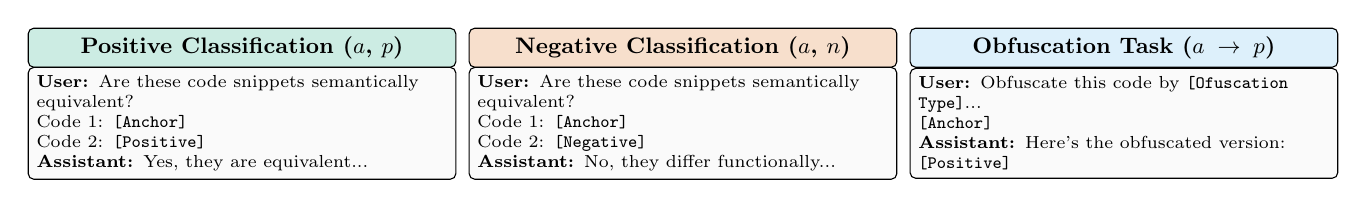
\begin{tikzpicture}[scale=0.8, every node/.style={scale=0.9}]
        \definecolor{poscolor}{RGB}{0,158,115}
        \definecolor{negcolor}{RGB}{213,94,0}
        \definecolor{gencolor}{RGB}{86,180,233}
        \definecolor{codebg}{RGB}{250,250,250}
        \definecolor{textgray}{gray}{0.15}

        % Positive Classification
        \node[draw, fill=poscolor!20, text width=5.8cm, align=center, font=\small\bfseries, rounded corners=2pt]
            at (-7, 5.2) {Positive Classification ($a$, $p$)};
        \node[draw, fill=codebg, text width=5.8cm, align=left, font=\scriptsize, rounded corners=2pt]
            at (-7, 4.0) {
            \textbf{User:} Are these code snippets semantically equivalent?\\
            Code 1: \texttt{[Anchor]}\\
            Code 2: \texttt{[Positive]}\\
            \textbf{Assistant:} Yes, they are equivalent...
        };

        % Negative Classification
        \node[draw, fill=negcolor!20, text width=5.8cm, align=center, font=\small\bfseries, rounded corners=2pt]
            at (0, 5.2) {Negative Classification ($a$, $n$)};
        \node[draw, fill=codebg, text width=5.8cm, align=left, font=\scriptsize, rounded corners=2pt]
            at (0, 4.0) {
            \textbf{User:} Are these code snippets semantically equivalent?\\
            Code 1: \texttt{[Anchor]}\\
            Code 2: \texttt{[Negative]}\\
            \textbf{Assistant:} No, they differ functionally...
        };

        % Forward Generation
        \node[draw, fill=gencolor!20, text width=5.8cm, align=center, font=\small\bfseries, rounded corners=2pt]
            at (7, 5.2) {Obfuscation Task ($a \rightarrow p$)};
        \node[draw, fill=codebg, text width=5.8cm, align=left, font=\scriptsize, rounded corners=2pt]
            at (7, 4.0) {
            \textbf{User:} Obfuscate this code by \texttt{[Ofuscation Type]}...\\
            \texttt{[Anchor]}\\
            \textbf{Assistant:} Here's the obfuscated version:\\
            \texttt{[Positive]}
        };
    \end{tikzpicture}
    \caption{The three distinct task formats used in Contrastive Fine-Tuning (CFT).}
    \label{fig:contrastive_prompting}
    \vspace{-0.45cm}
\end{figure*}

Whether the same reasoning-generation split holds for Dead Code Insertion and
Literal Encryption remains open. Those tasks demand more than token-level
substitution, and our prompts do not surface comparably explicit intermediate
mappings. The mechanism claim is therefore scoped. The lexical evidence is
direct, while the extension to structural and semantic inverses rests on the
shared behavioral endpoint together with the differing recovery profiles reported
next.


\subsection{Balanced Bidirectional Fine-Tuning}
\label{sec:bft}



Balanced bidirectional fine-tuning (BFT) trains on forward and reverse pairs at
once and therefore sets a recovery ceiling for the reverse task. Its results show
that standard fine-tuning does not erase reverse capability in any absolute
sense. Given explicit reverse supervision, the models recover much of the inverse
on Identifier Renaming and Dead Code Insertion. On the lexical transformation,
BFT reaches up to 80\% recovery, at a 59\% average across models. On the
structural transformation, it reaches 76\% at best, at a 52\% average.


The recovery registers on every reverse-direction metric. Against the SFT
endpoint, BFT raises identifier-set overlap with the original to 0.45.
It lowers $AST_{\text{struct}}$ between the deobfuscated output and the
obfuscated input to 0.37.
The outputs therefore move away from the obfuscated input and toward the
original code in both identifiers and structure. CodeBLEU and readability follow.
Readability rises by 0.29 in absolute terms over the SFT reverse output.
It does not reach the original readability of 0.79. BFT thus demonstrates
that the reverse task is not inherently impossible on the lexical and structural
cases, and that explicit reverse supervision re-opens that direction.



% Literal Encryption resists this treatment. Even with balanced reverse
% supervision, its reverse recovery stays at 0\%. We therefore treat Literal
% Encryption as a boundary case for the current methods rather than as evidence for
% a single mechanism. The failure could stem from the difficulty of autoregressive
% recovery of encrypted literals, from the enlarged inverse search space, or from a
% deeper interaction between fine-tuning and sequence generation. The defensible
% conclusion is operational. For data-flow inverses of this kind, explicit reverse
% supervision is insufficient under the present setup.


Literal Encryption resists this treatment. Even with balanced reverse
supervision, its reverse recovery stays at 0\%.
Under this task design, that endpoint is expected.
The model must recover AES-encrypted literals from hard-coded decryption
logic, not apply a local inverse mapping.
We therefore treat Literal Encryption as a semantic boundary case for the
current methods, not as proof of a generic reverse failure.
The defensible conclusion is operational.
For semantic inverses of this kind, explicit reverse supervision is
insufficient under the present setup.


\begin{table}[tb]
\centering
\caption{Consolidated reverse accuracies (\%) and forward accuracies in
parentheses across models, training strategies, and transformation types.
SFT (Fwd) is the forward pass rate before self-correction.
Post-correction rates appear in Section~\ref{sec:cognitive_specialization}
and Figure~\ref{fig:model_performance}.
$\Delta_{\text{BRF}}$ is the bidirectional gap under each strategy.}
\begin{adjustbox}{width=.7\columnwidth,center}
\label{tab:consolidated_results}
\begin{tabular}{@{}l cc cc cc cc@{}}
\toprule
& \multicolumn{2}{c}{\textbf{SFT}} & \multicolumn{2}{c}{\textbf{BFT}} & \multicolumn{2}{c}{\textbf{CFT}} & \multicolumn{2}{c}{$\Delta_{\text{BRF}}$} \\
\cmidrule(lr){2-3} \cmidrule(lr){4-5} \cmidrule(lr){6-7} \cmidrule(lr){8-9}
\textbf{Model} & Rev & (Fwd) & Rev & (Fwd) & Rev & (Fwd) & SFT & CFT \\
\midrule
\multicolumn{9}{l}{\textit{Identifier Renaming (IR)}} \\
\midrule
GPT-4.1-mini & 0 & (81) & 80 & (72) & 52 & (72) & 81 & 20 \\
GPT-3.5-Turbo & 0 & (76) & 72 & (70) & 48 & (68) & 76 & 20 \\
Qwen2.5-7B & 0 & (60) & 52 & (58) & 39 & (60) & 60 & 21 \\
Qwen2.5-Coder-7B & 0 & (65) & 55 & (64) & 43 & (65) & 65 & 22 \\
DeepSeek-R1-Distill-Qwen-7B & 0 & (63) & 48 & (56) & 36 & (56) & 63 & 20 \\
Mistral-7B & 0 & (68) & 49 & (60) & 41 & (62) & 68 & 21 \\
\midrule
\multicolumn{9}{l}{\textit{Dead Code Insertion (DCI)}} \\
\midrule
GPT-4.1-mini & 0 & (60) & 76 & (65) & 0 & (68) & 60 & 68 \\
GPT-3.5-Turbo & 0 & (53) & 58 & (62) & 0 & (60) & 53 & 60 \\
Qwen2.5-7B & 0 & (40) & 42 & (40) & 0 & (38) & 40 & 38 \\
Qwen2.5-Coder-7B & 0 & (48) & 45 & (44) & 0 & (46) & 48 & 46 \\
DeepSeek-R1-Distill-Qwen-7B & 0 & (45) & 38 & (38) & 0 & (34) & 45 & 34 \\
Mistral-7B & 0 & (73) & 55 & (52) & 0 & (52) & 73 & 52 \\
\midrule
\multicolumn{9}{l}{\textit{Literal Encryption (LE)}} \\
\midrule
GPT-4.1-mini & 0 & (22) & 0 & (28) & 0 & (26) & 22 & 26 \\
GPT-3.5-Turbo & 0 & (22) & 0 & (40) & 0 & (38) & 22 & 38 \\
Qwen2.5-7B & 0 & (12) & 0 & (14) & 0 & (12) & 12 & 12 \\
Qwen2.5-Coder-7B & 0 & (19) & 0 & (16) & 0 & (16) & 19 & 16 \\
DeepSeek-R1-Distill-Qwen-7B & 0 & (15) & 0 & (12) & 0 & (10) & 15 & 10 \\
Mistral-7B & 0 & (30) & 0 & (20) & 0 & (18) & 30 & 18 \\
\bottomrule
\end{tabular}
\end{adjustbox}
\end{table}
